\documentclass[../main.tex]{subfiles}

\begin{document}

\section{Extra work}

\subsection{Testing}
Before doing all these parallelizations, we decided that it would be nice to have some way of testing that, when changing the code, we wouldn't break it. So we decided to do some automatic tests.

These test consist in the comparison of the resulting heat image generated of the code executions of the same size and steps (we assume that the serial code results in a correct image). The implementation of these tests is in the \textit{run-tests.sh} file and can be run by running \textit{Code \ref{code:run-tests}}, which will result in an output similar to \textit{Figure \ref{fig:run-tests}}

\begin{code}[numbers=left]{title=Run tests,label=code:run-tests}{bash}
    $ make test
\end{code}

\begin{figure}[!htb]
    \centering
    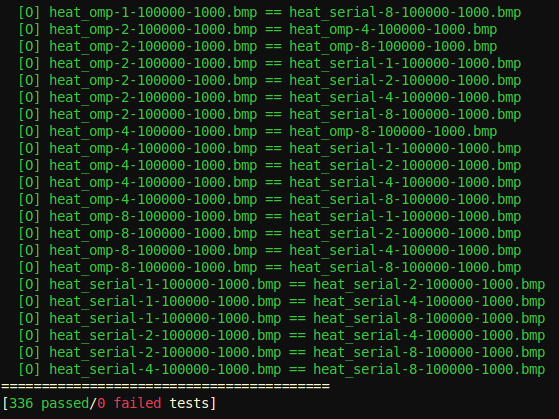
\includegraphics[width= 0.5\linewidth]{\subfix{../media/figures/test-results.png}}\
    \caption{Snippet of the resulting logs of running the tests}
    \label{fig:run-tests}
\end{figure}

\subsection{Batch running}

Before running these tests, we need a way of easily generating those images. To do so, we made `run-multiple-omp.sh', which implementation sets up all the variable combinations possible and submits them to the queue. To run these executions do it by running \textit{Code \ref{code:run-code}}

\begin{code}[numbers=left]{title=Run code,label=code:run-code}{bash}
    $ make [all | serial | omp]
\end{code}

Once these executions end, we can check it using `qstat', we can run the tests.

\subsection{Resulting time extraction}

Once the execution ends and the tests are passing, we have \textbf{PLENTY} of log files with the different resulting times and some other logs. To facilitate the extraction of time, we made `run-extract-time.sh', which can be called by running \textit{Code \ref{code:run-time}}.
Which will generate a `results.csv' with the resulting times and the information of the different executions to process further.

\begin{code}[numbers=left]{title=Run time extraction,label=code:run-time}{bash}
    $ make time
\end{code}

\end{document}